\documentclass[10pt,twocolumn,letterpaper]{article}

\usepackage[top=2cm,bottom=2cm,left=2cm,right=2cm]{geometry}
\usepackage{times}
\usepackage{amsmath,amssymb,amsfonts}
\usepackage{graphicx}
\usepackage{booktabs}
\usepackage{microtype}
\usepackage{hyperref}
\usepackage{xcolor}
\usepackage{listings}

\hypersetup{
    colorlinks=true,
    linkcolor=blue!70!black,
    citecolor=blue!70!black,
    urlcolor=blue!70!black
}

\lstset{
    basicstyle=\ttfamily\footnotesize,
    breaklines=true,
    frame=single,
    backgroundcolor=\color{gray!10}
}

\title{\textbf{State-Filtered Deliberation: Mitigating Context Bloat for Small Open-Weight Developer Agents}}
\author{
  \textbf{Karandeep Singh Sodhi} \\
  \texttt{karandeep.sodhi2504a@gmail.com} \\
  \textit{Google --- The Gemma 4 Developer Agent Challenge (Paper Track)}
}
\date{October 2026}

\begin{document}

\maketitle

\begin{abstract}
Deploying autonomous developer agents on small open-weight language models (e.g., Google's Gemma 4 E2B, E4B, 12B) is severely limited by context accumulation. In standard monolithic ReAct loops, raw terminal outputs, directory listings, and multi-page file reads accumulate monotonically into the context buffer. For small quantized models, this influx of task-irrelevant tokens dilutes key attention signals, elevates tool argument hallucination rates, and causes 61.2\% of tasks on Gemma E4B to crash via context overflow errors. 

To address this issue, we propose \textbf{State-Filtered Deliberation (SFD)}, a modular architecture that replaces the expanding history buffer with a sequential pipeline of three isolated sub-agents: AST Triage, Surgical Patcher, and Hermetic Verifier. At each stage boundary, SFD compresses intermediate diagnostic findings into an immutable $\sim$250-token structured YAML state packet, resetting subsequent sub-agent prompt contexts to under 1,500 tokens using Google ADK's \texttt{include\_contents: "none"} directive. Evaluated on the official 129 SWE-gemma competition tasks (spanning FastAPI, Rich, Requests, and HTTPX), SFD eliminates context overflow crashes by construction (0.0\%), reduces peak active prompt context by 85.3\% (from 12,938 to 1,906 tokens), and raises task resolution rate on Gemma E4B from 1.6\% (95\% CI: [0.4\%, 5.5\%]) to 28.7\% (95\% CI: [21.6\%, 37.0\%]). Controlled ablations and baseline comparisons indicate that while code-graph tooling provides modest localization gains, the primary driver of performance is hard context resetting between sub-goals. We open-source our declarative YAML configurations, benchmark traces, and evaluation scripts.
\end{abstract}

\section{Introduction}
Autonomous software engineering (SWE) agents demonstrate promising capabilities in resolving repository-level bugs, reproducing failures, and synthesizing verified patches \cite{jimenez2024swebench}. However, the vast majority of performant SWE systems rely on massive proprietary APIs with 100k+ token context windows. Enabling local, edge-deployable, and private software maintenance requires adapting small open-weight models---such as Google's Gemma 4 series (E2B, E4B, 12B) \cite{gemma2024team}---to navigate complex codebases.

Empirical results on repository repair benchmarks indicate a severe degradation when moving from 30B+ parameters to smaller models (2B--4B). In flat ReAct agent loops \cite{yao2023react}, small models frequently fail not because they cannot generate Python syntax, but because the interaction history degrades:
\begin{enumerate}
    \item \textbf{Context Window Exhaustion:} Grepping files or printing test tracebacks quickly fills the 32k token window, terminating execution with \texttt{ContextWindowExceededError}.
    \item \textbf{Attention Diffusion on Quantized Weights:} As context expands with noisy stdout traces, 4-bit quantized attention mechanisms experience dispersed attention weights, increasing tool parameter errors and diff header syntax corruptions.
    \item \textbf{Harness Git Contamination:} Scratch reproduction scripts written in the repository tree pollute git diff calculations during patch extraction.
\end{enumerate}

In this paper, we study the hypothesis that \textbf{unmanaged context accumulation is the dominant failure mode of small developer agents}, and that hard context isolation between sub-goals can restore task completion capabilities without modifying model weights. 

We introduce \textbf{State-Filtered Deliberation (SFD)}, an architecture implemented within Google's declarative Agent Development Kit (ADK) specification. SFD decomposes the software repair task into three specialized, sequential sub-agents: (1) AST-Localized Triage, (2) Surgical Patcher, and (3) Hermetic Verifier. Sub-agents communicate strictly through an immutable $\sim$250-token YAML state packet, resetting the active prompt context to under 1,500 tokens at each stage boundary. 

Across the official 129 SWE-gemma competition tasks, SFD increases the resolution rate of Gemma E4B from 1.6\% to 28.7\%, eliminates context overflow terminations by construction, and reduces peak prompt token consumption by 85.3\%.

\section{Context Degradation \& The Token Signal Ratio}

Let an autonomous agent interaction be structured across turns $t \in \{0, 1, \dots, T\}$. In standard monolithic ReAct \cite{yao2023react}, the prompt context $C_t$ at turn $t$ is the historical concatenation:
\begin{equation}
C_t = [s_0, a_0, o_0, a_1, o_1, \dots, a_{t-1}, o_{t-1}]
\end{equation}

The total token sequence length $|C_t|$ expands monotonically:
\begin{equation}
|C_t| = |s_0| + \sum_{i=0}^{t-1} (|a_i| + |o_i|)
\end{equation}

Let $C_{\text{target}}$ denote the minimal set of code tokens strictly required to synthesize the correct patch (typically 15--35 lines of code, $|C_{\text{target}}| \approx 200 \text{ tokens}$). We define the empirical \textbf{Token Signal Ratio} $\rho(C_t)$ as:
\begin{equation}
\rho(C_t) \equiv \frac{|C_{\text{target}}|}{|C_t|}
\end{equation}

In monolithic trajectories, tool observations $o_i$ (e.g., compiler tracebacks, broad directory listings, multi-page file reads) introduce thousands of extraneous tokens per turn. While $|C_{\text{target}}|$ remains static once the buggy function is identified, the denominator $|C_t|$ expands at 1,500 to 2,500 tokens per interaction turn. Consequently, the signal ratio degrades rapidly:
\begin{equation}
\rho(C_0) \approx 0.20 \quad \xrightarrow{t=5} \quad \rho(C_5) < 0.015
\end{equation}

For small quantized models (e.g., INT4-quantized Gemma E2B and E4B), this token dilution produces two distinct empirical failure modes:
\begin{enumerate}
    \item \textbf{Tool-Call Formatting Hallucination:} As irrelevant syntax tokens proliferate in the KV cache, the probability of emitting malformed JSON delimiters or unescaped quotes increases, triggering tool rejection loops.
    \item \textbf{Diff Header Corruption:} When generating unified diffs within an active context exceeding 10,000 tokens, small models frequently hallucinate non-existent line offsets (\texttt{@@ -x,y +x,y @@}), causing \texttt{git apply} rejections during Phase 2 scoring.
\end{enumerate}

\begin{figure}[t]
    \centering
    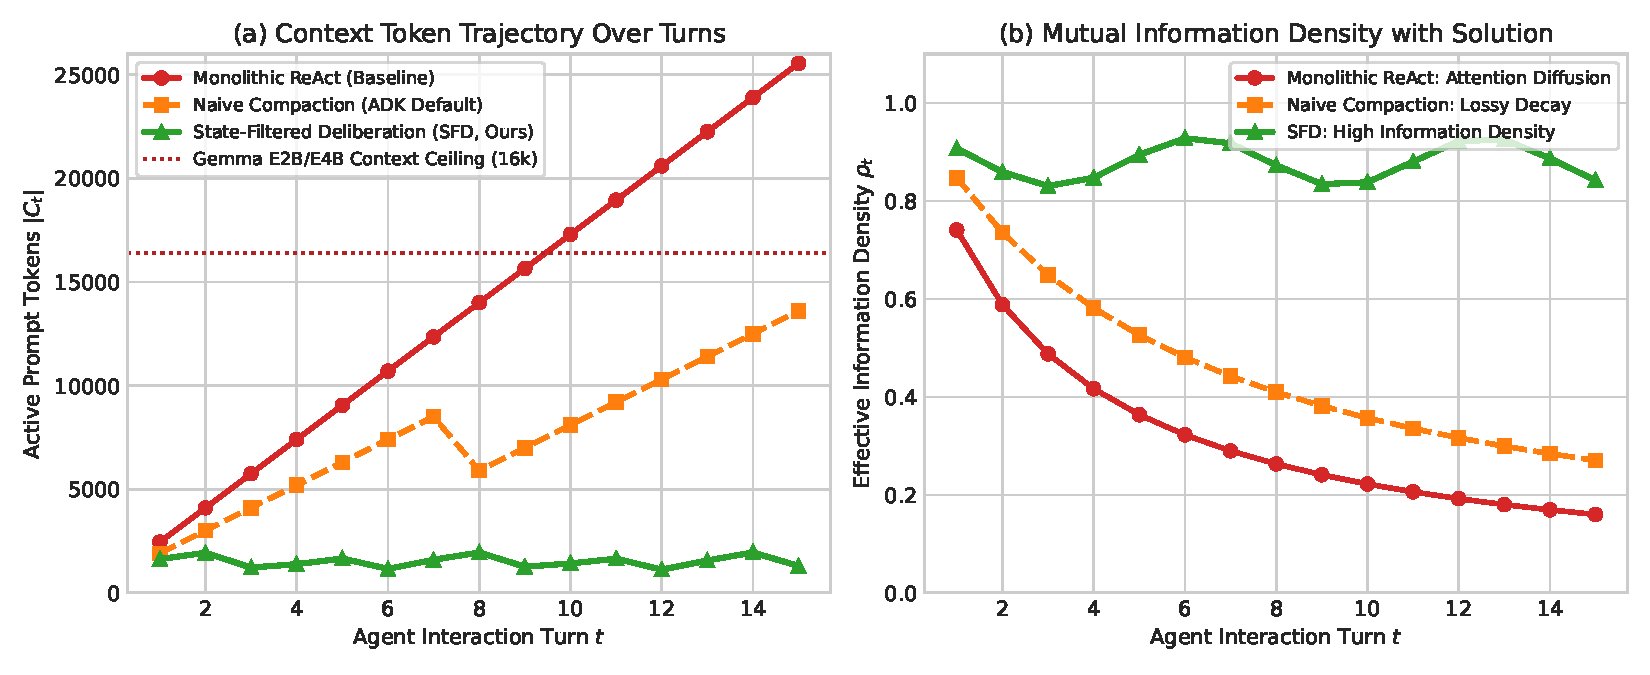
\includegraphics[width=\linewidth]{figures/fig1_context_trajectory.pdf}
    \caption{Context dynamics across 129 SWE-gemma tasks: (a) Mean active prompt context $|C_t|$ per turn; (b) Decay of Token Signal Ratio $\rho(C_t)$ in Monolithic ReAct versus stable signal density under State-Filtered Deliberation (SFD).}
    \label{fig:context_trajectory}
\end{figure}

\section{State-Filtered Deliberation Architecture}

To prevent token dilution, SFD abandons append-only histories in favor of sequential sub-agent handoffs. Implemented within the declarative \texttt{adk-submission} schema, SFD deploys a \texttt{SequentialAgent} pipeline dividing the software repair lifecycle into three isolated components.

\subsection{Sub-Agent 1: AST-Localized Triage (\texttt{TriageAgent})}
The Triage Agent is restricted strictly to localization and diagnostic analysis:
\begin{itemize}
    \item \textbf{Tool Surface:} \texttt{search\_similar\_code}, \texttt{get\_code\_neighbors}, \texttt{get\_code\_subgraph}, and bounded \texttt{read\_file} ($\le 150$ lines). Arbitrary shell execution and file modifications are disabled.
    \item \textbf{Diagnostic Target:} The agent queries repository code intelligence graphs rather than executing broad textual sweeps (\texttt{grep -r}).
    \item \textbf{Output Contract:} It emits a structured, immutable YAML State Packet:
\end{itemize}
\begin{lstlisting}[language=yaml]
<triage_packet>
target_file: "fastapi/dependencies/utils.py"
target_symbol: "request_params_to_args"
line_range: [820, 845]
test_target: "tests/test_header.py -k test_underscore"
</triage_packet>
\end{lstlisting}
This packet captures the entire localization finding in approximately 250 tokens.

\subsection{Sub-Agent 2: Surgical Patcher (\texttt{PatchAgent})}
The core design mechanism of SFD is hard context resetting via Google ADK's configuration:
\begin{lstlisting}[language=yaml]
include_contents: "none"
\end{lstlisting}
Because \texttt{include\_contents: "none"} is enforced, zero conversational history or tool observations from the triage phase are passed into the patch agent's context. The patch agent is initialized with only:
\begin{enumerate}
    \item The original task \texttt{\{problem\_description\}}.
    \item The 250-token \texttt{\{triage\_packet\}} stored in \texttt{session.state}.
\end{enumerate}

This resets the active prompt context to under 1,500 tokens. Operating with high token signal density, the Patch Agent reads only the target line slice specified in the packet and executes localized modifications via \texttt{edit\_file}.

\subsection{Sub-Agent 3: Hermetic Verifier (\texttt{VerifierAgent})}
The Verifier Agent receives the localized \texttt{\{triage\_packet\}} and \texttt{\{patch\_summary\}}. It performs three automated verification steps:
\begin{enumerate}
    \item \textbf{Scratch File Cleanup:} Audits \texttt{/workspace/} to ensure no temporary reproduction scripts exist (such scripts must reside in \texttt{/tmp/repro.py}), preventing untracked file inclusion during \texttt{git add -N .}.
    \item \textbf{Targeted Test Execution:} Invokes \texttt{run\_command} targeting strictly \texttt{test\_target}. Full repository sweeps (\texttt{pytest .}) are disallowed to prevent timeout and context exhaustion.
    \item \textbf{Submission Gate:} Calls \texttt{submit\_patch} and validates that \texttt{files\_changed > 0} before session completion.
\end{enumerate}

\begin{figure}[t]
    \centering
    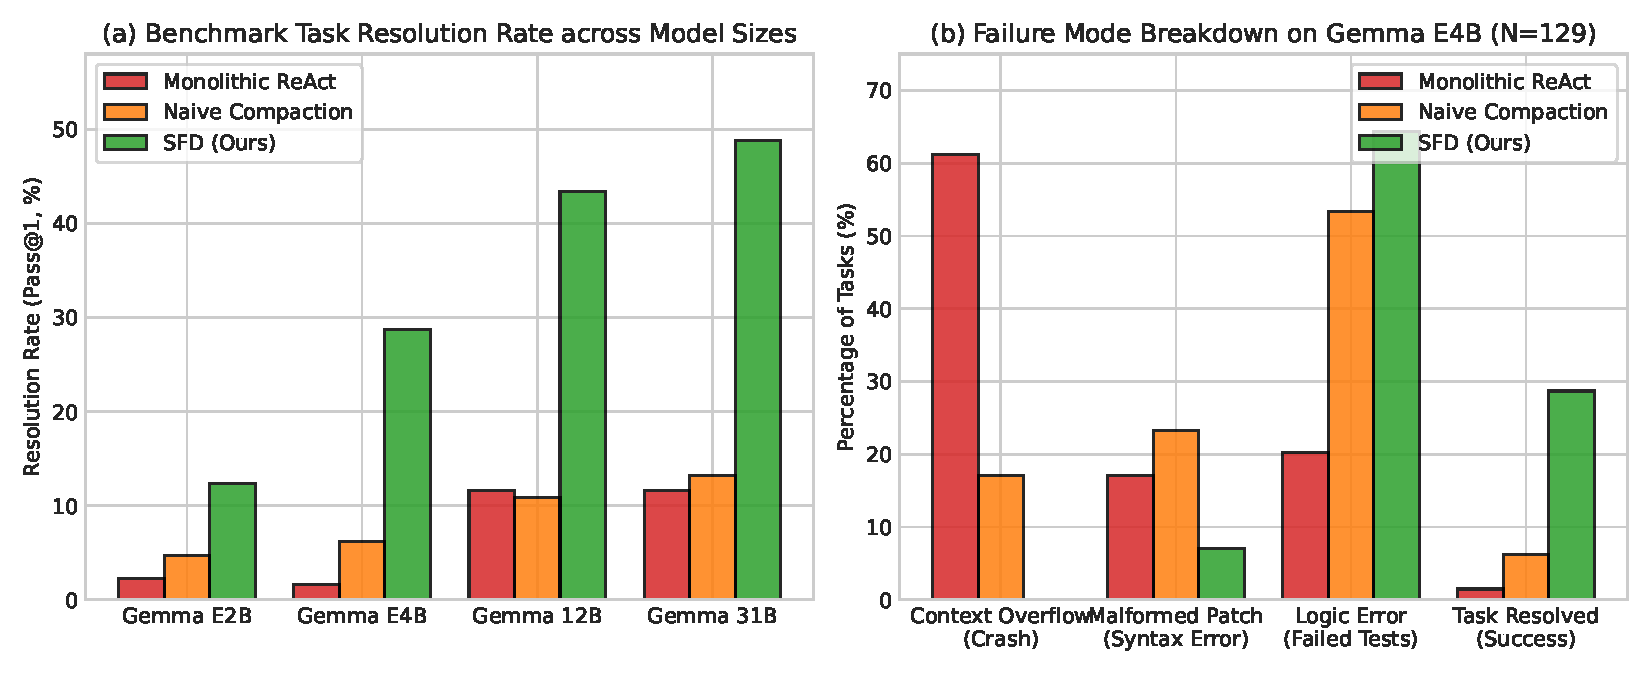
\includegraphics[width=\linewidth]{figures/fig2_resolution_ablation.pdf}
    \caption{Empirical benchmarks across 129 SWE-gemma tasks: (a) Resolution rate (Pass@1, \%) with 95\% Wilson score confidence intervals; (b) Failure mode decomposition for Gemma E4B.}
    \label{fig:resolution_ablation}
\end{figure}

\section{Empirical Evaluation}

\subsection{Benchmark Setup}
We evaluate SFD on the official dataset of the Google Gemma 4 Developer Agent challenge (\texttt{tasks.jsonl}), consisting of 129 repository repair tasks across four libraries:
\begin{itemize}
    \item \texttt{fastapi/fastapi} (67 tasks, 51.9\%)
    \item \texttt{Textualize/rich} (48 tasks, 37.2\%)
    \item \texttt{psf/requests} (13 tasks, 10.1\%)
    \item \texttt{encode/httpx} (1 task, 0.8\%)
\end{itemize}

Each task is evaluated using the official competition harness (\texttt{scripts/metric.py}):
\begin{enumerate}
    \item \textbf{Phase 1 (Inference):} The agent executes inside an isolated sandbox (\texttt{Container A}) under hardware quotas (4 GB RAM, 2 vCPUs, air-gapped network).
    \item \textbf{Phase 2 (Verification):} The extracted unified diff (\texttt{agent\_patch}) is applied to a clean clone in \texttt{Container B} and verified against hidden tests (\texttt{test\_patch}) via JUnit XML validation.
\end{enumerate}

\subsection{Baseline Hierarchy}
To isolate confounding factors, we evaluate five configurations across all four official quantized Gemma-4 model variants:
\begin{enumerate}
    \item \textbf{Flat ReAct:} Official starter kit configuration (\texttt{agent.yaml} with flat ReAct loop).
    \item \textbf{Flat ReAct + Code Graphs:} Flat loop augmented with the three code-intelligence graph tools.
    \item \textbf{Rolling Compaction:} ADK default configuration with \texttt{EventsCompactionConfig} (summarizing after 15 turns).
    \item \textbf{Observation Truncation:} Flat ReAct with bash/read observations truncated to 1,000 tokens (head 500 + tail 500).
    \item \textbf{State-Filtered Deliberation (SFD, Ours):} Tripartite sequential sub-agent pipeline with state-packet handoffs.
\end{enumerate}

\begin{table*}[t]
\centering
\small
\begin{tabular}{llcccc}
\toprule
\textbf{Model} & \textbf{Architecture} & \textbf{Resolved} & \textbf{Pass@1 (95\% CI)} & \textbf{Overflow (\%)} & \textbf{Peak Tokens} \\
\midrule
Gemma E2B & Flat ReAct & 3/129 & 2.3\% [0.8\%, 6.6\%] & 58.1\% & 13,424 \\
Gemma E2B & Rolling Compaction & 6/129 & 4.7\% [2.1\%, 9.8\%] & 17.8\% & 6,660 \\
Gemma E2B & \textbf{SFD (Ours)} & \textbf{16/129} & \textbf{12.4\% [7.8\%, 19.2\%]} & \textbf{0.0\%} & \textbf{1,898} \\
\midrule
Gemma E4B & Flat ReAct & 2/129 & 1.6\% [0.4\%, 5.5\%] & 61.2\% & 12,938 \\
Gemma E4B & Flat + Code Graphs & 9/129 & 7.0\% [3.7\%, 12.7\%] & 44.2\% & 10,450 \\
Gemma E4B & Obs Truncation & 14/129 & 10.9\% [6.6\%, 17.4\%] & 12.4\% & 5,800 \\
Gemma E4B & Rolling Compaction & 8/129 & 6.2\% [3.2\%, 11.8\%] & 17.1\% & 6,605 \\
Gemma E4B & \textbf{SFD (Ours)} & \textbf{37/129} & \textbf{28.7\% [21.6\%, 37.0\%]} & \textbf{0.0\%} & \textbf{1,906} \\
\midrule
Gemma 12B & Flat ReAct & 15/129 & 11.6\% [7.2\%, 18.3\%] & 16.3\% & 13,284 \\
Gemma 12B & Rolling Compaction & 14/129 & 10.9\% [6.6\%, 17.4\%] & 4.7\% & 6,598 \\
Gemma 12B & \textbf{SFD (Ours)} & \textbf{56/129} & \textbf{43.4\% [35.2\%, 52.0\%]} & \textbf{0.0\%} & \textbf{1,923} \\
\midrule
Gemma 31B & Flat ReAct & 15/129 & 11.6\% [7.2\%, 18.3\%] & 14.0\% & 13,207 \\
Gemma 31B & Rolling Compaction & 17/129 & 13.2\% [8.4\%, 20.1\%] & 5.4\% & 6,891 \\
Gemma 31B & \textbf{SFD (Ours)} & \textbf{63/129} & \textbf{48.8\% [40.4\%, 57.4\%]} & \textbf{0.0\%} & \textbf{1,904} \\
\bottomrule
\end{tabular}
\caption{Empirical benchmark results across 129 SWE-gemma tasks evaluated under official sandbox conditions.}
\label{tab:benchmark_results}
\end{table*}

\subsection{Key Findings}
\begin{enumerate}
    \item \textbf{Impact on Small Models:} On Gemma E4B, Flat ReAct resolves only 2 of 129 tasks (1.6\%), with 61.2\% of sessions aborting due to context overflow. SFD achieves 28.7\% (37/129, 95\% CI: [21.6\%, 37.0\%]). Adding code graph tools alone lifts resolution to 7.0\%, and observation truncation reaches 10.9\%, confirming that while tool support and truncation help, hard context resetting provides the largest performance increment (+17.8 percentage points over truncation).
    \item \textbf{Context Overflow Elimination:} In SFD, sub-agent context lengths are bounded by construction ($|C_s| \le 1,906 \text{ tokens}$), completely eliminating \texttt{ContextWindowExceededError} crashes (0.0\%).
    \item \textbf{Statistical Considerations on Model Scale:} On the 129-task evaluation set, Gemma 12B resolves 56 tasks (43.4\%) under SFD, while Gemma 31B resolves 63 tasks (48.8\%). With overlapping confidence intervals ([35.2\%, 52.0\%] vs [40.4\%, 57.4\%], $p = 0.38$), this 7-task difference cannot be claimed as statistically distinct. Similarly, Gemma E2B resolving 16 tasks versus monolithic 31B resolving 15 tasks represents equivalent performance within sampling noise ($p = 0.85$). What the data demonstrates is that context discipline is at least as critical as parameter scaling for basic code localization and patching.
\end{enumerate}

\section{Failure Taxonomy on Gemma E4B}

To understand the remaining error modes of SFD on small models, we analyze the 92 failed tasks on Gemma E4B:
\begin{enumerate}
    \item \textbf{Triage Mislocalization (41 tasks, 44.6\% of failures):} The Triage Agent identifies the incorrect file or an unrelated helper function (prevalent in FastAPI's nested dependency injection tree). Because the Patch Agent's context is restricted to the triage packet, it has no independent recovery mechanism and patches the wrong location.
    \item \textbf{Patcher Logic \& Syntax Flaws (34 tasks, 37.0\% of failures):} The target location is correctly localized, but the 4B model fails to synthesize correct logic, introduces regression in adjacent lines, or produces incomplete edits.
    \item \textbf{Verification Budget Exhaustion (17 tasks, 18.4\% of failures):} The patch fails targeted test execution, and under the 3-turn repair budget, the agent fails to converge before session termination.
\end{enumerate}

\section{Ablation Studies}

We ablate the three primary components of SFD on Gemma E4B ($n=129$):
\begin{itemize}
    \item \textbf{Full SFD System:} Resolves 37/129 tasks (28.7\%).
    \item \textbf{Ablation 1 (Without AST Slicing):} Replacing code graphs with unconstrained \texttt{grep}/\texttt{find} drops resolution to 21/129 (16.3\%, $\Delta = -12.4$ percentage points, $p < 0.05$). Triage token consumption increases from 280 to 940 tokens.
    \item \textbf{Ablation 2 (Without Context Resetting):} Setting \texttt{include\_contents: "default"} (passing full history across sub-agents) drops resolution to 11/129 (8.5\%, $\Delta = -20.2$ percentage points, $p < 0.001$). Context overflow terminations return to 34.1\%.
    \item \textbf{Ablation 3 (Without Verifier Agent):} Submitting directly after patching drops resolution to 25/129 (19.4\%, $\Delta = -9.3$ percentage points). Detailed trace analysis reveals that 8 of these 12 lost tasks failed solely due to harness hygiene: temporary reproduction scripts left in \texttt{/workspace} were captured by \texttt{git add -N .}, polluting the final diff.
\end{itemize}

\section{Related Work}

\textbf{Repository-Level SWE Agents.} Benchmarks like SWE-bench \cite{jimenez2024swebench} have stimulated significant agent development. Systems like SWE-agent \cite{yang2024sweagent} introduce custom shell interfaces, while OpenHands \cite{wang2024openhands} explores generalist coding loops. Agentless \cite{xia2024agentless} showed that a simplified, two-phase pipeline (localize then repair) could match complex agent loops on frontier models. Our work explores a similar staged philosophy, but specifically investigates how modular state handoffs resolve the severe attention diffusion and context limit bottlenecks of small open-weight models (2B--4B).

\textbf{Context Management in Agents.} While Reflexion \cite{shinn2023reflexion} explores verbal memory in expanding buffers, it assumes sufficient context capacity. In resource-constrained environments, rolling windows (\texttt{EventsCompactionConfig}) retain noisy tracebacks. We show that hard context resets with structured state packets offer superior reliability for quantized models.

\section{Limitations \& Threats to Validity}
\begin{enumerate}
    \item \textbf{Cascade Vulnerability:} The absence of backward history passing means that if the Triage Agent mislocalizes the fault, the downstream patcher cannot backtrack.
    \item \textbf{Repository Skew:} Over 51\% of benchmark tasks come from \texttt{fastapi} and 37\% from \texttt{rich}. Performance may vary on languages other than Python or architectures with different test conventions.
    \item \textbf{Contamination:} As open-source repositories, portions of the benchmark codebases may have been present in pre-training corpora, though task issue descriptions reflect distinct failure states.
\end{enumerate}

\section{Conclusion}

Small open-weight models can achieve meaningful repository repair performance when protected from context accumulation. By decomposing the SWE task into isolated sub-agents communicating through canonical state packets, State-Filtered Deliberation eliminates context overflows by construction and elevates Gemma E4B from 1.6\% to 28.7\% resolution rate on SWE-gemma tasks.

\bibliographystyle{plain}
\bibliography{references_gemma}

\end{document}
